% CS 6501 3D Computer Vision -- Final Project Report (CVPR style, 8 pages + references)
\documentclass[10pt,twocolumn,letterpaper]{article}
\usepackage[pagenumbers]{cvpr}
\usepackage{cuted}
\usepackage{caption}
\usepackage{graphicx}
\graphicspath{{figures/}}
\usepackage{booktabs}
\usepackage{multirow}
\usepackage{amsmath,amssymb}
\usepackage{microtype}
\definecolor{cvprblue}{rgb}{0.21,0.49,0.74}
\usepackage[pagebackref,breaklinks,colorlinks,allcolors=cvprblue]{hyperref}
\def\confName{CVPR}
\def\confYear{2027}
\usepackage{xspace}
\newcommand{\dB}{\,dB\xspace}
\newcommand{\cm}{\,cm\xspace}
\newcommand{\step}[1]{\textbf{(#1)}}
\newcommand{\new}[1]{\textbf{[#1]}}
% user-study numbers: fill in from the 'votes' collection before submission (search for \pending)
\newcommand{\pending}[1]{\textcolor{red}{#1}}

\title{Open Free-Viewpoint Reconstruction of Athletes with Dynamic 3D Gaussians}
\author{Faizan Khan\\ University of Virginia\\ {\tt\small xdy6sg@virginia.edu}}

\begin{document}
\twocolumn[{%
\renewcommand\twocolumn[1][]{#1}%
\maketitle
\vspace{-2.2em}
\begin{center}
  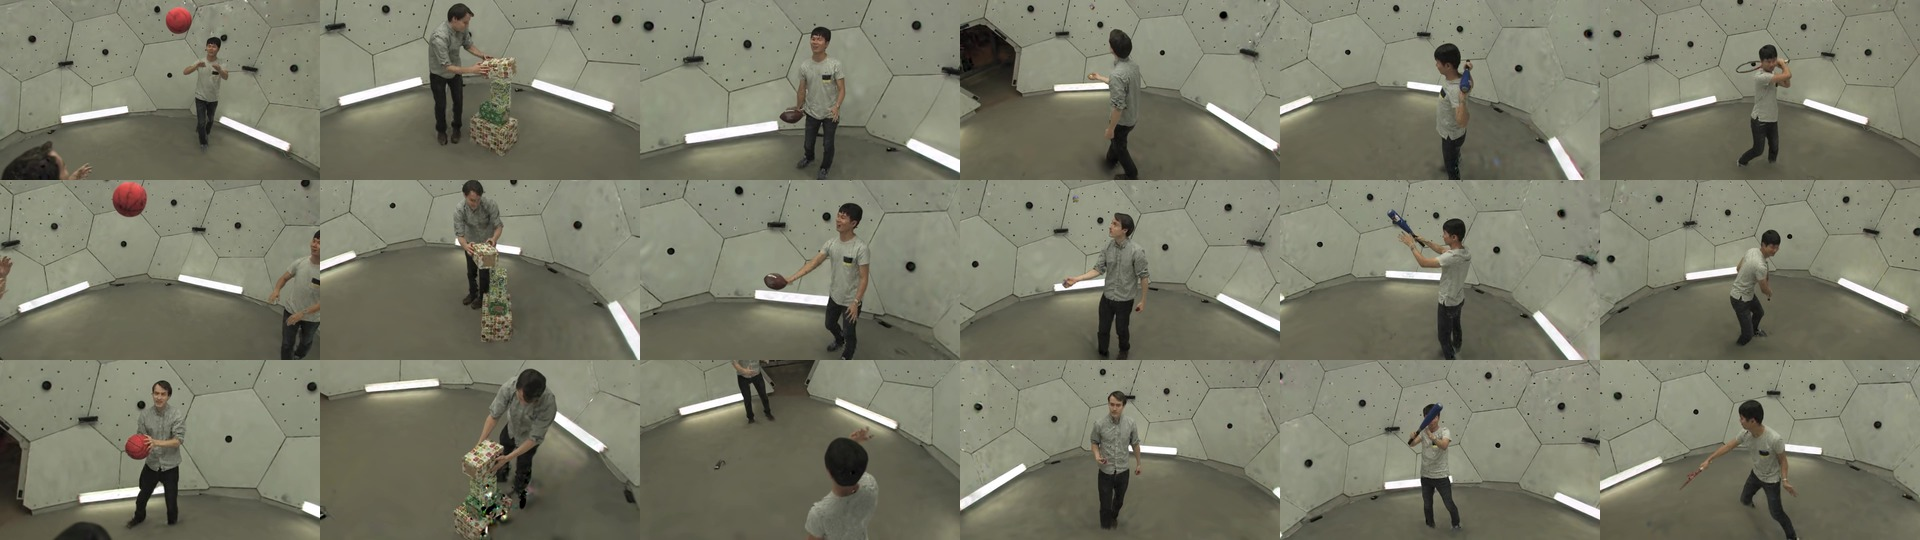
\includegraphics[width=\textwidth]{teaser.jpg}
  \vspace{-1.6em}
  \captionof{figure}{\textbf{Cinematic 3D replays made by our open pipeline.} Columns: basketball, boxes, football, juggle, softball, tennis. Rows: three moments of one automatically planned shot (push-in, freeze-time sweep, crane). Every 4D model was trained by us, and no real camera stood at any of these viewpoints.}
  \label{fig:teaser}
\end{center}
\vspace{0.4em}
}]

\begin{abstract}
Some sports broadcasts now show replays where time stops and the camera flies around the athlete. The systems behind them are closed, so it is hard to see how they work or how good they are. We build an open version. The input is synchronized multi-angle video; the output is a cinematic 3D replay with a free viewpoint, slow motion and freeze-time. The pipeline prepares the data, builds a 4D model with Dynamic 3D Gaussians (D3G), measures it, and hands it to an automatic ``director'' that plans the camera move. On top of this baseline we add three things: (A) a key-moment finder driven by 3D body skeletons, (B) a camera path that knows which way the athlete faces, and (C) cubic interpolation of the Gaussians between frames. We train all six PanopticSports clips ourselves. The models reach 27.0--28.7\dB PSNR on views they never saw and follow the athletes' joints to 2--5\cm (median). Cubic interpolation beats the straight-line blend in every sport, by up to 1.5\dB on the athlete. The full director never flies into a player, is 1,800$\times$ smoother than a naive orbit, and the facing-aware path cuts back views by up to a third. An ablation shows what each rule buys and where the old rules failed.
\end{abstract}

%%%%%%%%%%%%%%%%%%%%%%%%%%%%%%%%%%%%%%%%%%%%%%%%%%%%%%%%%%%%%%%%%%%%%%
\section{Introduction}
\label{sec:intro}

A replay that can freeze time and move the camera anywhere shows things the real cameras missed: the release of a throw, the angle of a bat, a foot on a line. In class we saw World Labs' Atlas~\cite{worldlabs2026atlas}, which turns ``a handful of ordinary cameras into a bullet time multiview capture studio.'' Arcturus~\cite{arcturus} sells this idea to broadcasters: synchronized sensors around a venue, a radiance field for every moment stored as splats, and new views from any position. Online, an engineer at Roboflow rebuilds players as textured 3D bodies from a single broadcast camera~\cite{mirrash2026b,mirrash2026}, building on Roboflow's open tools for player tracking~\cite{skalski2025roboflow}, and another posted a Gaussian splat of a World Series home run~\cite{middlecamp2026}. \cref{fig:insp} shows these sources.

None of them releases a full pipeline from video to replay, and none reports accuracy. We first tried the single-camera route ourselves. The new views looked plausible, but we could not check them, because no other camera saw the scene. So we moved to synchronized multi-view video, where cameras held out from training give real images to compare against.

\noindent\textbf{Goal.} Given synchronized multi-angle video of athletes, produce an immersive, cinematic 3D replay, and measure how faithful it is. Uses include broadcasting, coaching and AR/VR.

\noindent\textbf{What is new since the mid-term.} The mid-term built the baseline (v6): our own basketball model, released models for the other clips, and a rule-based director. Three weak spots stood out: the ``ball'' rule froze at the wrong moment (in \emph{boxes} it tracked red wrapping paper), some shots started behind the athlete, and slow motion cut corners on curved motion. This report fixes each one and tests every claim:
\begin{itemize}\itemsep0pt
\item \textbf{One setup for all results.} We trained all six clips ourselves, and measured 3D accuracy against motion-capture skeletons, not just images.
\item \textbf{(A) Skeleton-driven key moment.} We align the dataset's 3D skeletons to every clip and freeze at the peak wrist speed of the most active athlete.
\item \textbf{(B) Facing-aware camera path.} The director picks the side and sweep direction that keep the camera in front of the athlete.
\item \textbf{(C) Cubic interpolation.} In-between Gaussians follow a Catmull-Rom curve~\cite{catmull1974} instead of a straight line.
\item \textbf{Experiments and analysis.} An ablation of every director rule, an ablation of D3G's physical priors, an in-between-frame test against real images, an error analysis, and a viewer study.
\end{itemize}

\begin{figure}[t]
\centering
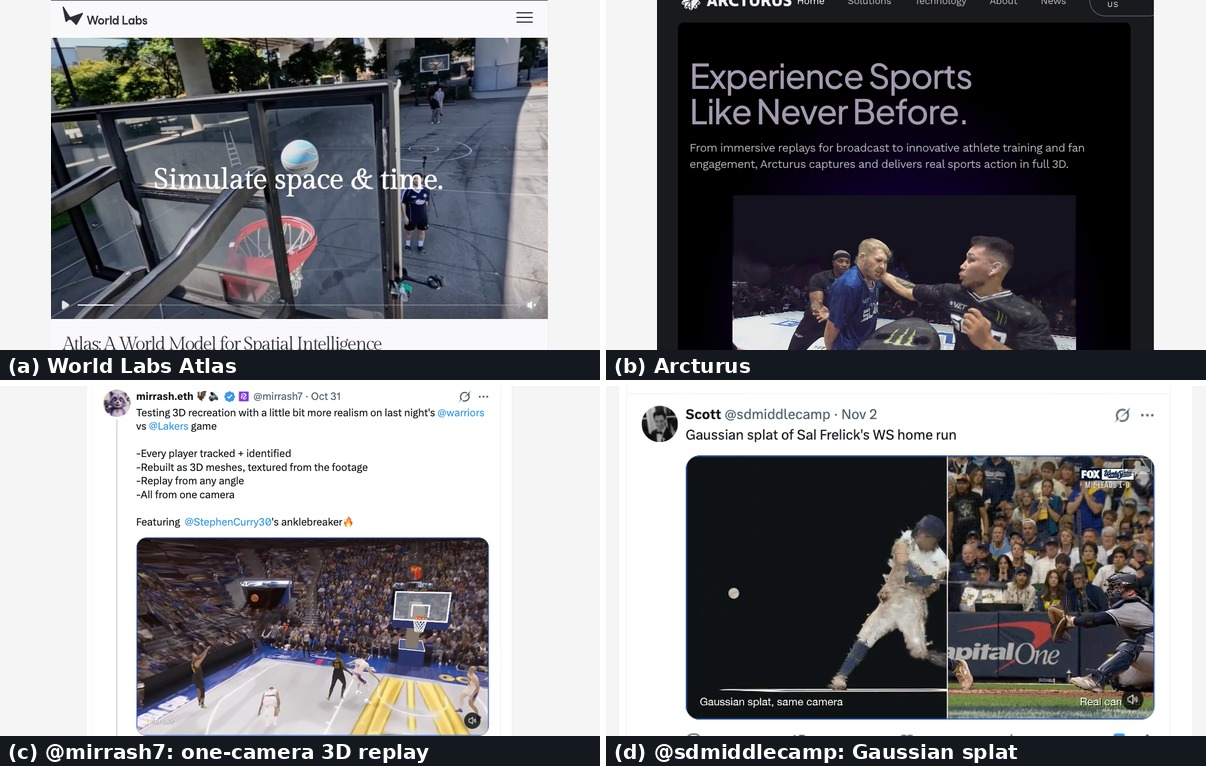
\includegraphics[width=\columnwidth]{inspiration.jpg}
\vspace{-1.6em}
\caption{\textbf{What inspired this project.} (a) World Labs' Atlas, shown in class~\cite{worldlabs2026atlas}. (b) Arcturus, volumetric sports replays for broadcast~\cite{arcturus}. (c) A 3D replay rebuilt from one broadcast camera~\cite{mirrash2026b}. (d) A Gaussian splat of a World Series home run~\cite{middlecamp2026}. Screenshots, Nov.\ 2026.}
\label{fig:insp}
\vspace{-1em}
\end{figure}

%%%%%%%%%%%%%%%%%%%%%%%%%%%%%%%%%%%%%%%%%%%%%%%%%%%%%%%%%%%%%%%%%%%%%%
\section{Background and Related Work}
\label{sec:related}

\noindent\textbf{Radiance fields and splatting.} NeRF~\cite{mildenhall2020nerf} stores a scene in a neural network and renders it by volume rendering. 3D Gaussian Splatting (3DGS)~\cite{kerbl3dgs} stores it as millions of small 3D Gaussians and renders them in real time, which suits video. Both need calibrated cameras; in a real venue these come from structure-from-motion such as COLMAP~\cite{schoenberger2016sfm}.

\noindent\textbf{Dynamic scenes.} D3G~\cite{luiten2024dynamic} keeps one set of Gaussians for the whole clip and moves them frame by frame, with physical priors that keep neighbours moving together. Because its Gaussians persist, it also tracks every point in 3D. 4DGS~\cite{wu20244dgs} and Spacetime Gaussians~\cite{li2024spacetime} model motion with a deformation field or per-Gaussian curves. D4RT~\cite{zhang2025d4rt} and CoTracker3~\cite{karaev2024cotracker3} recover depth and motion from video in one pass, but do not aim at photoreal new views.

\noindent\textbf{Feed-forward reconstruction.} VGGT~\cite{wang2025vggt} and MapAnything~\cite{keetha2025mapanything} predict cameras and geometry from images in one pass; RayZer~\cite{jiang2025rayzer} and WildRayZer~\cite{chen2026wildrayzer} learn view synthesis without 3D labels; pixelSplat~\cite{charatan2024pixelsplat}, MVSplat~\cite{chen2024mvsplat} and FSGS~\cite{zhu2024fsgs} build splats from few images. Such models may one day replace our per-clip optimization.

\noindent\textbf{Sports and camera planning.} The CMU Panoptic Studio~\cite{joo2015panoptic} provides our data and its skeletons. Sports vision mostly targets tracking and pose~\cite{somers2024soccernet,jiang2024worldpose,skalski2025roboflow}, not photoreal views. For camera motion we borrow two classic tools: Catmull-Rom splines~\cite{catmull1974} and quaternion curves for rotations~\cite{shoemake1985}.

%%%%%%%%%%%%%%%%%%%%%%%%%%%%%%%%%%%%%%%%%%%%%%%%%%%%%%%%%%%%%%%%%%%%%%
\section{Dataset: PanopticSports}
\label{sec:data}

PanopticSports was released with D3G~\cite{luiten2024dynamic}. It is cut from capture \texttt{161029\_sports1} of the CMU Panoptic Studio~\cite{joo2015panoptic}, a geodesic dome lined with cameras. It has six clips of one or two people: \emph{basketball} (two players passing), \emph{boxes} (stacking boxes), \emph{football} (throwing an American football), \emph{juggle}, \emph{softball} (swinging a bat) and \emph{tennis} (swinging a racket). Each clip has 150 synchronized frames per view at 640$\times$360, camera calibration, foreground masks and a starting point cloud. A fixed set of views is held out for testing only; these have no masks.

\noindent\textbf{Skeletons.} The raw capture also has 3D body skeletons (19 joints per person) from Panoptic's own multi-view pose system~\cite{cao2017openpose,joo2015panoptic}. The clips do not say where in the capture they start, so we align them ourselves (\cref{sec:skel}). We use the skeletons in two ways: as ground truth for 3D motion, and as cues for the director.

%%%%%%%%%%%%%%%%%%%%%%%%%%%%%%%%%%%%%%%%%%%%%%%%%%%%%%%%%%%%%%%%%%%%%%
\section{Method}
\label{sec:method}

\begin{figure*}[t]
\centering
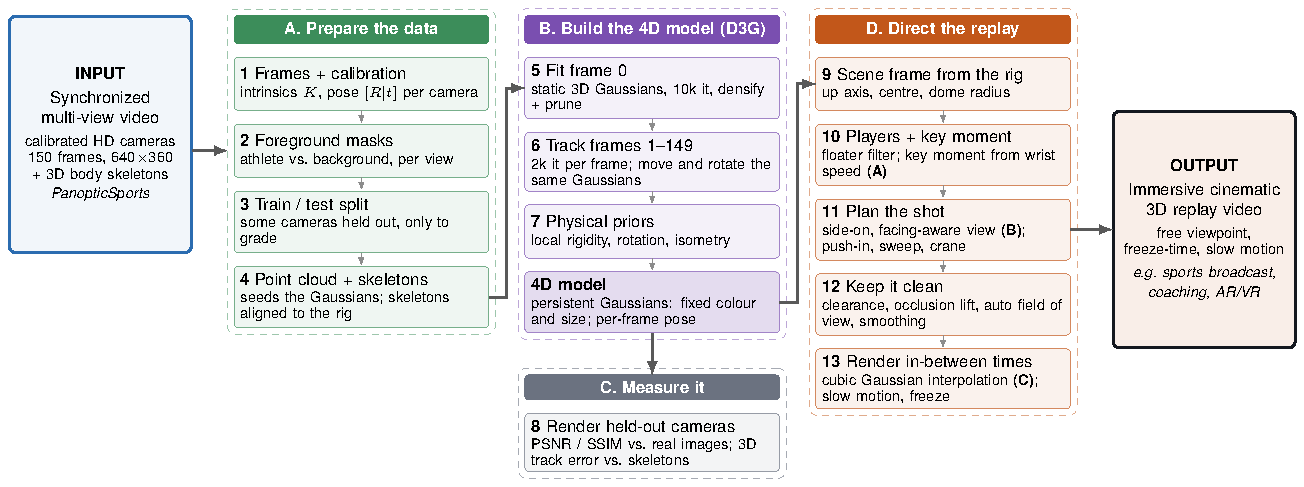
\includegraphics[width=\textwidth]{workflow.pdf}
\vspace{-1.6em}
\caption{\textbf{Workflow.} Synchronized multi-view video goes through four stages. A: prepare frames, calibration, masks, a train/test split, a starting point cloud and aligned skeletons. B: build the 4D model with Dynamic 3D Gaussians. C: measure it on held-out views and against the skeletons. D: the director plans and renders the replay. (A), (B) and (C) in bold mark this report's three additions.}
\label{fig:workflow}
\vspace{-0.6em}
\end{figure*}

\begin{figure*}[t]
\centering
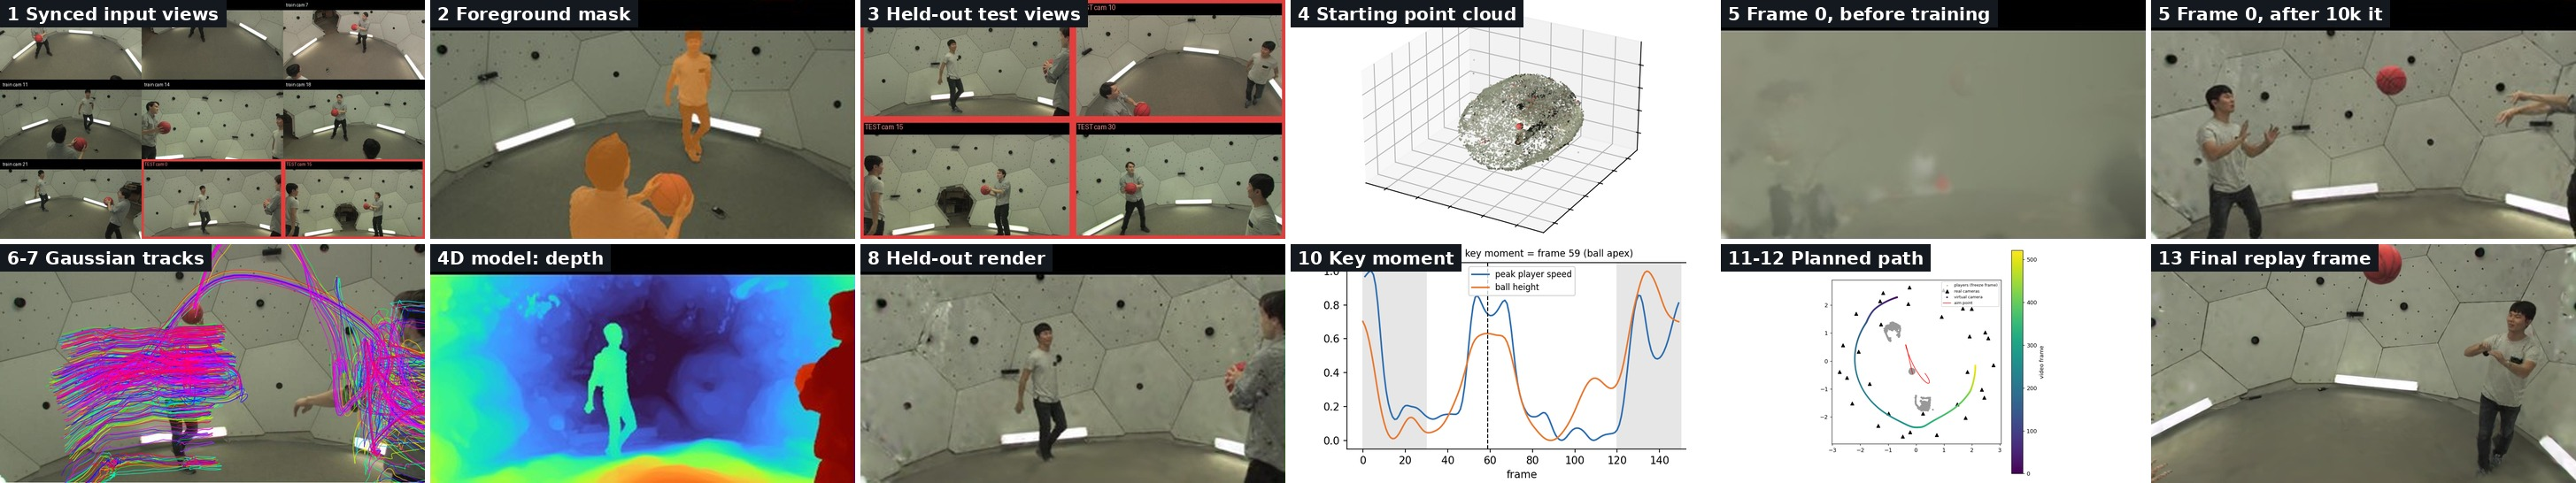
\includegraphics[width=\textwidth]{stages.jpg}
\vspace{-1.6em}
\caption{\textbf{Intermediate output after each step} (basketball). Numbers refer to the steps in \cref{fig:workflow}. Step 3 shows the held-out test views (red). Step 10 plots normalized ball height and peak player speed (the v6 cues that (A) replaces).}
\label{fig:stages}
\vspace{-1em}
\end{figure*}

\cref{fig:workflow} shows the whole workflow and \cref{fig:stages} what comes out of each step. We first summarize the baseline from the mid-term, then describe the three additions.

\subsection{Baseline pipeline (v6)}
\noindent\textbf{A. Prepare the data.} \step{1} We load each camera's intrinsics $K$ and pose. \step{2} Foreground masks separate the athletes from the dome; D3G learns an athlete/background label on every Gaussian from them. \step{3} Held-out views are never used for training and only grade the result. \step{4} Each Gaussian starts at one point of the released cloud (194k points).

\noindent\textbf{B. Build the 4D model.} \step{5} Frame 0 is fit like static 3DGS for 10k iterations with an $\ell_1$+SSIM image loss and a mask loss, growing to 330--365k Gaussians. \step{6} Each later frame starts from the previous one and gets 2k iterations; only position and rotation change. \step{7} Three priors keep this motion physical~\cite{luiten2024dynamic}: neighbours move \emph{rigidly} together, \emph{rotate} together, and keep their distances (\emph{isometry}). We kept D3G's loss weights (rigid 4, rotation 4, isometry 2) but made each one a command-line switch for the ablation in \cref{sec:priors}.

\noindent\textbf{C. Measure it.} \step{8} We render every held-out view at every frame and compare with the real image (PSNR, SSIM), and we compare 3D tracks with the skeletons (\cref{sec:q2}).

\noindent\textbf{D. Direct the replay.} \step{9} From the rig alone we recover the up direction, the point all optical axes meet, the dome radius $R$ and a band of safe camera heights. \step{10} Players are athlete-labelled Gaussians in dense clusters; stray ``floaters'' are dropped. v6 froze at the top of a red ``ball'', or else at peak motion. \step{11} We look across the main direction of motion so a throw is seen side-on, and fly a shot list: push-in, a 5\,s freeze-time sweep of 130$^\circ$, a crane and a settle. \step{12} The camera keeps $\ge 0.35R$ from every player, rises if a player blocks the view, widens its lens to fit the play, and its aim is smoothed twice. \step{13} For slow motion (0.4$\times$) and freeze-time we render Gaussians \emph{between} frames. Output is 17\,s at 1280$\times$720, 30\,fps.

\subsection{Aligning the skeletons}
\label{sec:skel}
The skeletons live in Panoptic's world (centimetres); D3G uses its own world. Both share the same cameras, so we fit a similarity transform $(s,\mathbf{R},\mathbf{t})$ between the two sets of camera centres with Umeyama's method~\cite{umeyama1991}. The fit is exact (residual ${<}10^{-9}$, $s=0.01$, i.e.\ D3G units are metres). To find each clip's start frame, we project the skeletons of every candidate start into the training views and keep the start where the most joints land inside the foreground masks. Every clip reaches a 100\% hit rate (\cref{fig:skel}), at raw frames 4061 (basketball), 8503 (boxes), 2186 (football), 5202 (juggle), 535 (softball) and 830 (tennis).

\begin{figure}[t]
\centering
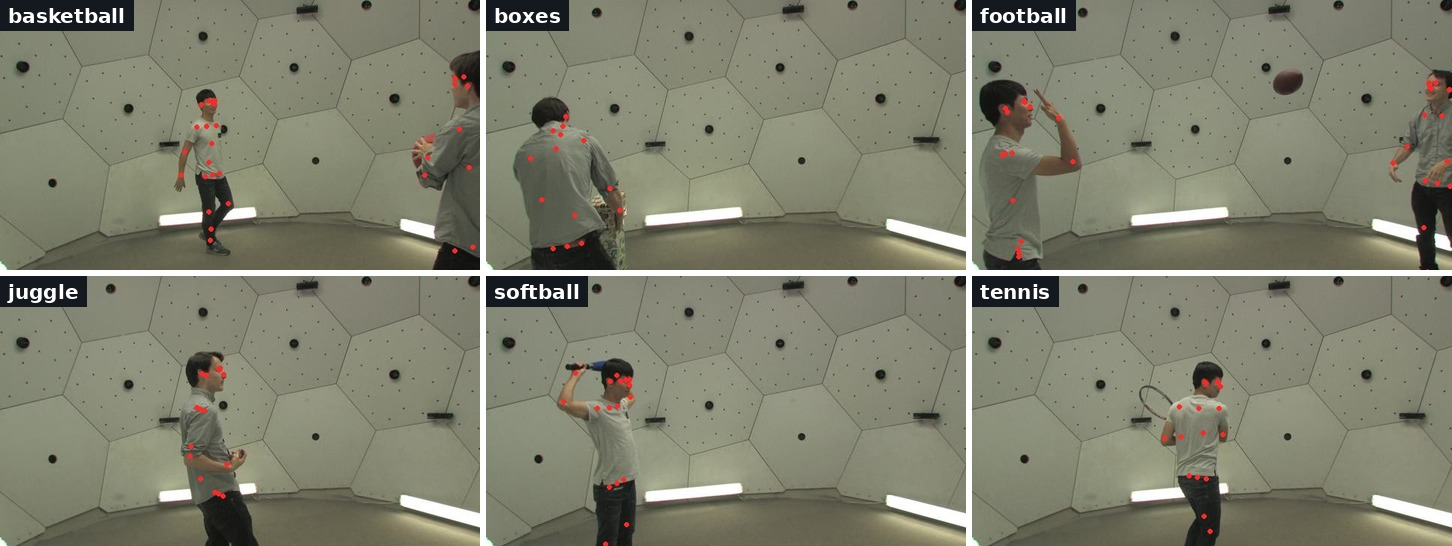
\includegraphics[width=\columnwidth]{skeletons.jpg}
\vspace{-1.6em}
\caption{\textbf{Aligned skeletons} projected into a training view, one clip per tile. Every joint lands on the athlete, which checks both the alignment and the calibration.}
\label{fig:skel}
\vspace{-1em}
\end{figure}

\subsection{(A) Key moment from the skeletons}
For every athlete $b$ we compute the speed of the faster wrist, $v_b(t)=\max_{w}\lVert \mathbf{J}_{b,w}(t)-\mathbf{J}_{b,w}(t{-}1)\rVert$, and smooth it with a Gaussian ($\sigma{=}2$ frames). The key athlete is the one with the highest peak inside the middle of the clip, $t\in[0.2T,0.8T]$, and the freeze frame is that peak. The window keeps the freeze away from the clip ends, where the push-in and settle need room. Wrist speed peaks at the release of a throw or the contact of a swing, which is what a replay wants to stop on, and it works with no ball at all.

\subsection{(B) Facing-aware camera path}
From the key athlete's hips and shoulders we get a torso normal, and the nose and eyes fix its sign; projected onto the floor, this is the facing direction $\mathbf{f}(t)$. v6 picked the side-on view and the sweep direction by rule, so in \emph{football} and \emph{juggle} the replay opened on the athlete's back. Now the director tries both side-on views ($\pm90^\circ$ from the motion) and both sweep directions, plans the full path for each of the four, and keeps the one with the fewest frames ``behind'' the athlete, where the view direction is more than $110^\circ$ from $\mathbf{f}(t)$. Ties go to the v6 choice, so (B) only changes a shot when it helps.

\subsection{(C) Cubic interpolation between frames}
Slow motion and freeze-time need the scene at fractional times $t{+}u$, $u\in(0,1)$. v6 blended each Gaussian's position and colour linearly between frames $t$ and $t{+}1$, and its rotation by a normalized quaternion blend. A straight line cuts the corner of a curved path: a swinging bat or a ball arc. We use a Catmull-Rom curve through four frames instead,
\begin{equation}
\begin{aligned}
\mathbf{x}(u)=\tfrac12\big[\,&2\mathbf{p}_1+(\mathbf{p}_2{-}\mathbf{p}_0)\,u+(2\mathbf{p}_0{-}5\mathbf{p}_1{+}4\mathbf{p}_2{-}\mathbf{p}_3)\,u^2\\
&+(3\mathbf{p}_1{-}\mathbf{p}_0{-}3\mathbf{p}_2{+}\mathbf{p}_3)\,u^3\big]
\end{aligned}
\end{equation}
with $\mathbf{p}_i$ the positions at frames $t{-}1,\dots,t{+}2$. It passes exactly through every reconstructed frame and has a continuous velocity. For rotations we first flip each quaternion onto the same hemisphere as its neighbour ($\mathbf{q}$ and $-\mathbf{q}$ are the same rotation), apply the same curve, and normalize~\cite{shoemake1985}. Colours stay linear. At the clip ends the missing neighbour is repeated.

%%%%%%%%%%%%%%%%%%%%%%%%%%%%%%%%%%%%%%%%%%%%%%%%%%%%%%%%%%%%%%%%%%%%%%
\section{Experiments}
\label{sec:exp}

\noindent\textbf{Setup.} All six models are ours, trained with the same code and settings on the UVA HPC cluster (A100, A40, A6000 and newer GPUs; about 3 hours per clip, under 1\,GB of GPU memory). All image scores use the held-out views, which training never saw. We ask six questions. \textbf{Q1} Do the models match real views they never saw? \textbf{Q2} Do they capture the athletes' true 3D motion? \textbf{Q3} Does cubic interpolation give better in-between frames? \textbf{Q4} Does the skeleton find the right moment? \textbf{Q5} What does each director rule buy? \textbf{Q6} Which replay do viewers prefer? A last part asks which D3G priors matter.

\subsection{Q1: held-out image quality}
Our models score 27.0--28.7\dB PSNR and 0.89--0.91 SSIM on held-out views (\cref{tab:q1q2}, \cref{fig:heldout}). On the five clips with released models we are 0.3--1.2\dB lower (0.65\dB on average). We used the same code, settings and seed, so we put most of this gap down to run-to-run noise: in \cref{sec:priors}, four basketball runs that are identical up to frame 0 already differ by 1.2\dB at frame 0. Newer library versions and different GPUs add to it. In every clip PSNR drops by about 1\dB from the well-fit frame 0 and then holds steady.

\begin{figure}[t]
\centering
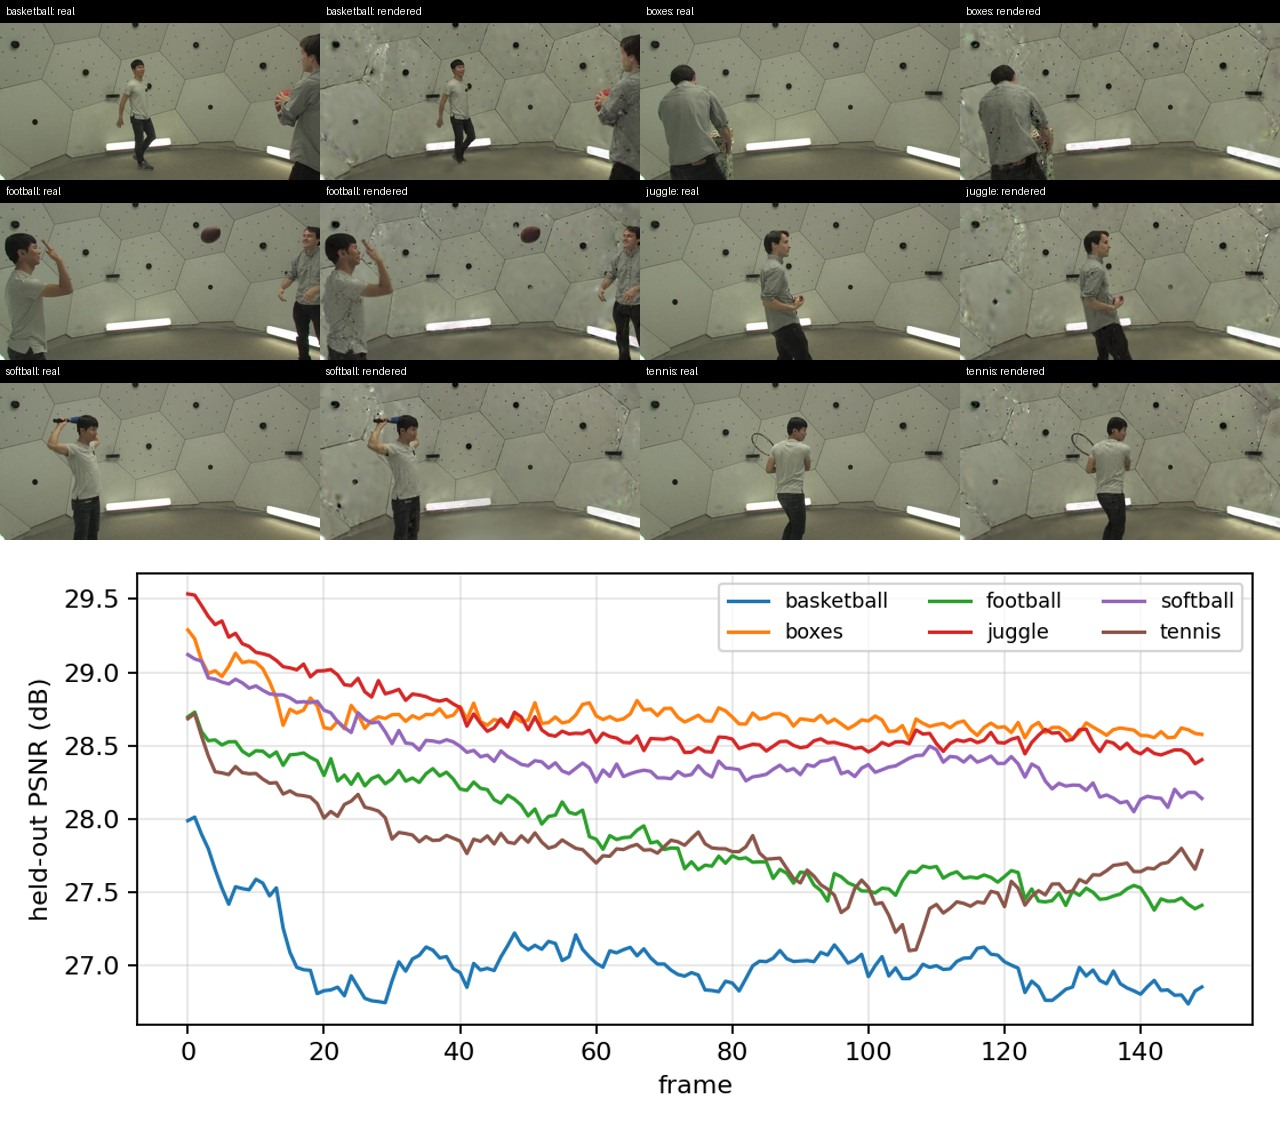
\includegraphics[width=\columnwidth]{heldout_ours.jpg}
\vspace{-1.6em}
\caption{\textbf{Q1: held-out views, our models.} Top: real vs.\ rendered held-out view for all six sports. Bottom: held-out PSNR for every frame.}
\label{fig:heldout}
\vspace{-1em}
\end{figure}

\begin{table}[t]
\centering\small
\setlength{\tabcolsep}{2.6pt}
\begin{tabular}{lccc|cccc}
\toprule
& \multicolumn{3}{c|}{Q1: held-out view} & \multicolumn{4}{c}{Q2: 3D track error (cm)}\\
Clip & PSNR & SSIM & released & mean & med. & ${<}5$\cm & static\\
\midrule
basketball & 27.03 & 0.891 & -- & 9.22 & 3.66 & 67\% & 97.3\\
boxes & 28.70 & 0.902 & 29.01 & 4.11 & 3.45 & 83\% & 33.2\\
football & 27.88 & 0.899 & 29.03 & 6.09 & 2.02 & 88\% & 30.8\\
juggle & 28.67 & 0.907 & 29.28 & 3.80 & 1.95 & 82\% & 53.7\\
softball & 28.43 & 0.903 & 28.78 & 4.32 & 3.10 & 69\% & 54.3\\
tennis & 27.78 & 0.903 & 28.60 & 5.76 & 5.22 & 47\% & 47.8\\
\bottomrule
\end{tabular}
\vspace{-0.6em}
\caption{\textbf{Q1 and Q2 across sports}, all models ours. ``Released'' is the D3G authors' model (PSNR). Track error: how far a Gaussian's 3D motion strays from the true joint motion, over all frames and joints; ``static'' is a model that never moves.}
\label{tab:q1q2}
\vspace{-1em}
\end{table}

\subsection{Q2: true 3D motion}
\label{sec:q2}
Images alone cannot tell whether the Gaussians move with the body or just look right from the cameras. The skeletons can. For every joint, the athlete Gaussians within 6\cm of it at its first visible frame are its \emph{anchors}. We follow the anchors through the 4D model and compare their \emph{displacement} with the joint's true displacement. We compare displacement, not position, because anchors sit on skin and clothes, not at the joint centre. The baseline is a model that never moves, whose error is simply how far the joint travels.

The models follow the body closely: median error is 2--5\cm in every sport, against 31--97\cm for the static model (\cref{tab:q1q2}). Torso and head are tracked to about 2--7\cm everywhere. Arms are the weak spot in the two ball sports (25\cm in basketball, 21\cm in football, against 3.5--8\cm elsewhere). The reason is visible in \cref{fig:tracks}: when a player catches or throws, some ``hand'' anchors are really ball Gaussians, which leave with the ball. Tennis has the highest median (5.2\cm): the racket and fast arm pull nearby anchors along.

\begin{figure}[t]
\centering
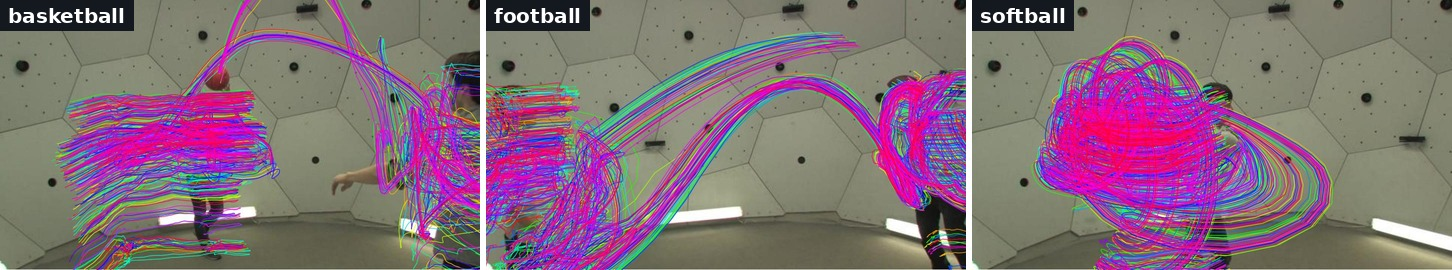
\includegraphics[width=\columnwidth]{tracks_ours.jpg}
\vspace{-1.6em}
\caption{\textbf{Q2: 3D tracks} of moving Gaussians over 150 frames, seen from a held-out view (basketball, football, softball).}
\label{fig:tracks}
\vspace{-1em}
\end{figure}

\subsection{Q3: in-between frames}
\label{sec:q3}
The slow-motion replay is made of in-between frames, but no real camera recorded those instants, so we cannot score them directly. Instead we \emph{hide} frames: we keep every $g$-th reconstructed frame ($g=2,4,8$), rebuild the hidden ones by interpolation, render the held-out views and compare with the real images, which do exist at those frames. This is the same problem at a larger gap. We compare frame repeat (nearest), the v6 straight-line blend, our cubic curve, and the model's own frame as the upper bound. The static dome fills most of the image and hides the difference, so we also score the athlete alone, using the model's rendered athlete mask, dilated by 5\,px.

Cubic beats linear in every sport and at every gap (\cref{tab:q3}). The gain grows with the gap, from 0.2\dB at $g{=}2$ to 1.0\dB at $g{=}8$ on average, and is largest in \emph{softball} (1.4--1.5\dB), whose bat swings in a tight arc. At $g{=}4$ cubic closes 59\% of the gap between linear and the real model. Frame repeat is far behind (up to 6\dB on the athlete). \cref{fig:interp} shows why: the straight-line blend leaves a ghost of the ball and racket between two positions, while the cubic curve keeps one sharp object.

\begin{table}[t]
\centering\small
\setlength{\tabcolsep}{3.4pt}
\begin{tabular}{lcccc|c}
\toprule
& \multicolumn{4}{c|}{athlete PSNR, $g{=}8$} & cubic$-$linear\\
Clip & repeat & linear & cubic & model & $g{=}2/4/8$\\
\midrule
basketball & 18.80 & 22.27 & \textbf{23.39} & 25.87 & +0.15/0.71/1.12\\
boxes & 23.07 & 24.71 & \textbf{25.30} & 26.30 & +0.02/0.31/0.60\\
football & 20.91 & 23.66 & \textbf{24.68} & 26.98 & +0.13/0.58/1.02\\
juggle & 20.90 & 24.07 & \textbf{24.66} & 26.98 & +0.13/0.50/0.59\\
softball & 19.46 & 22.33 & \textbf{23.79} & 27.46 & +0.41/1.41/1.46\\
tennis & 19.29 & 21.54 & \textbf{22.59} & 25.78 & +0.49/1.11/1.05\\
\midrule
mean & 20.41 & 23.09 & \textbf{24.07} & 26.56 & +0.22/0.77/0.98\\
\bottomrule
\end{tabular}
\vspace{-0.6em}
\caption{\textbf{Q3: in-between frames} scored against real held-out images, on the athlete only. Every $g$-th frame is kept and the rest rebuilt. ``Model'' uses the reconstructed frame itself (upper bound).}
\label{tab:q3}
\vspace{-1em}
\end{table}

\begin{figure}[t]
\centering
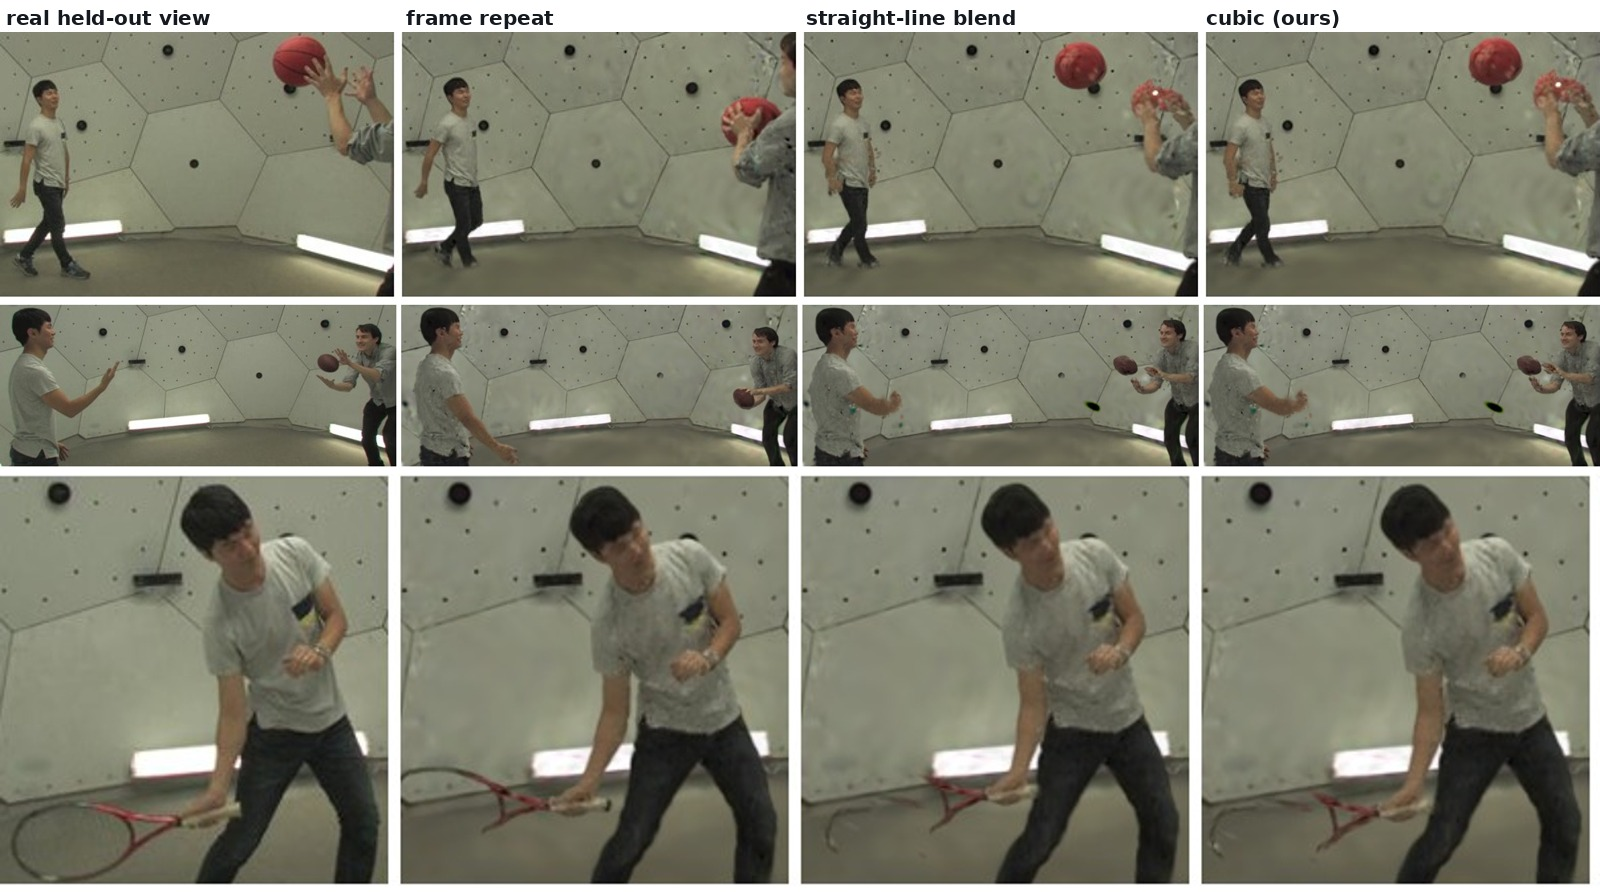
\includegraphics[width=\columnwidth]{interp_crops.jpg}
\vspace{-1.6em}
\caption{\textbf{Q3: a hidden frame rebuilt three ways} ($g{=}8$; basketball, football, tennis). The straight-line blend ghosts the ball and racket; cubic keeps them in one place.}
\label{fig:interp}
\vspace{-1em}
\end{figure}

\subsection{Q4: finding the key moment}
We labelled the decisive instant of each clip by hand from contact sheets (release of a pass or throw, contact of a swing, box set down), to about $\pm2$ frames. \emph{Juggle} is continuous and has no single moment, so it is left out. \cref{tab:q4} compares three rules. The v6 ball rule is more than 50 frames off in football, softball and tennis (median 51), and in \emph{boxes} it is close only by luck, since it tracked red wrapping paper. Both motion rules land within 3 frames in basketball, football and tennis. Neither finds the softball contact (frame 132), because it falls outside the middle-of-clip window; both stop at frames 87--89 instead. \emph{Boxes} is the hardest: the hands probably move fastest when lifting a box, not when placing it. Peak Gaussian motion is about as good as the skeleton here (median error 3 vs.\ 10), so the skeleton's real gain is that it says \emph{who} the key athlete is and which way they face, which (B) needs.

\begin{table}[t]
\centering\small
\setlength{\tabcolsep}{3.6pt}
\begin{tabular}{lc|ccc}
\toprule
& & \multicolumn{3}{c}{error (frames)}\\
Clip & label & ball (v6) & peak motion & skeleton (A)\\
\midrule
basketball & 53 & 6 & 0 & 10\\
boxes & 63 & 12 & 33 & 33\\
football & 66 & 53 & 1 & 2\\
softball & 132 & 51 & 45 & 43\\
tennis & 103 & 53 & 3 & 3\\
\midrule
mean / median & & 35 / 51 & 16.4 / 3 & 18.2 / 10\\
\bottomrule
\end{tabular}
\vspace{-0.6em}
\caption{\textbf{Q4: freeze frame vs.\ a hand label.} Both motion cues beat the ball rule; neither reaches the late softball contact.}
\label{tab:q4}
\vspace{-1em}
\end{table}

\subsection{Q5: what each director rule buys}
\label{sec:q5}
We switch off one rule at a time and plan the replay for all six sports. Planning needs no rendering, so the ablation is cheap and exact. We score each path on six numbers. \emph{Clip}: frames where the camera is closer than the clearance to a player. \emph{Occluded}: frames where a player blocks the line of sight to the aim point. \emph{Cut}: frames where less than 95\% of the action is in the picture. \emph{Behind}: frames where the camera is more than $110^\circ$ from where the key athlete faces. \emph{Eye jerk}: the third difference of the camera position per frame ($\times10^3/R$). \emph{Rot.\ jerk}: the same for the view direction, in degrees. The naive orbit blends the real camera poses at a similar speed.

\cref{tab:q5} gives the means. Every rule earns its place, and each one fixes the problem it was written for. Without clearance the camera flies into a player in 2.3\% of frames (13.6\% in basketball). Without the occlusion lift a player blocks the view in 1.9\% (11.5\% in football). Without the auto field of view half the frames cut off the action. Without smoothing the path is 1,400$\times$ jerkier. The full director is 1,800$\times$ smoother than the naive orbit, which also cuts off the action in 40\% of frames and spends 36\% of the time behind the athlete. The floater filter changes nothing on our models, which have few floaters. It mattered on the mid-term models (\cref{fig:versions}), so we keep it as a safety net.

Facing-awareness (B) lowers ``behind'' from 25.1\% to 21.0\% on average. The gain is all in the three clips where v6 opened on the athlete's back: football 36.3$\to$24.9\%, juggle 34.7$\to$28.0\%, softball 35.2$\to$29.0\%. The other three are unchanged, as designed. Compared with v6 as a whole, the full director has zero clipping (v6 0.3\%) and fewer back views (21.0 vs.\ 27.7\%). It costs a little framing (cut 14.9 vs.\ 11.7\%) and rare occlusion (0.3\%), because the new key moments fall in busier parts of the clip. \cref{fig:path} shows the planned path for basketball.

\begin{table}[t]
\centering\small
\setlength{\tabcolsep}{2.5pt}
\begin{tabular}{lcccccc}
\toprule
& clip & occl. & cut & behind & eye jerk & rot.\ jerk\\
Variant & \% & \% & \% & \% & max & max ($^\circ$)\\
\midrule
\textbf{full (A+B)} & \textbf{0.00} & 0.32 & 14.9 & \textbf{21.0} & 0.039 & 0.002\\
v6 (mid-term) & 0.31 & 0.00 & 11.7 & 27.7 & 0.032 & 0.002\\
\midrule
$-$ floater filter & 0.00 & 0.22 & 14.9 & 21.0 & 0.039 & 0.002\\
$-$ clearance & 2.26 & 0.32 & 14.9 & 20.9 & 0.035 & 0.002\\
$-$ occlusion lift & 0.00 & 1.91 & 14.9 & 21.0 & 0.032 & 0.002\\
$-$ auto field of view & 0.00 & 0.32 & 51.2 & 21.0 & 0.039 & 0.002\\
single smoothing & 0.00 & 0.22 & 14.9 & 21.1 & 0.188 & 0.077\\
no smoothing & 0.00 & 0.22 & 16.2 & 21.2 & 52.9 & 2.17\\
fixed view & 0.22 & 0.00 & 19.9 & 27.8 & 0.034 & 0.002\\
$-$ facing (B) & 0.00 & 0.16 & 14.9 & 25.1 & 0.041 & 0.002\\
\midrule
naive orbit & 0.61 & 4.10 & 40.0 & 36.3 & 70.2 & 3.31\\
\bottomrule
\end{tabular}
\vspace{-0.6em}
\caption{\textbf{Q5: director ablation}, mean over six sports (lower is better). Each row switches off one rule of the full director.}
\label{tab:q5}
\vspace{-1em}
\end{table}

\begin{figure}[t]
\centering
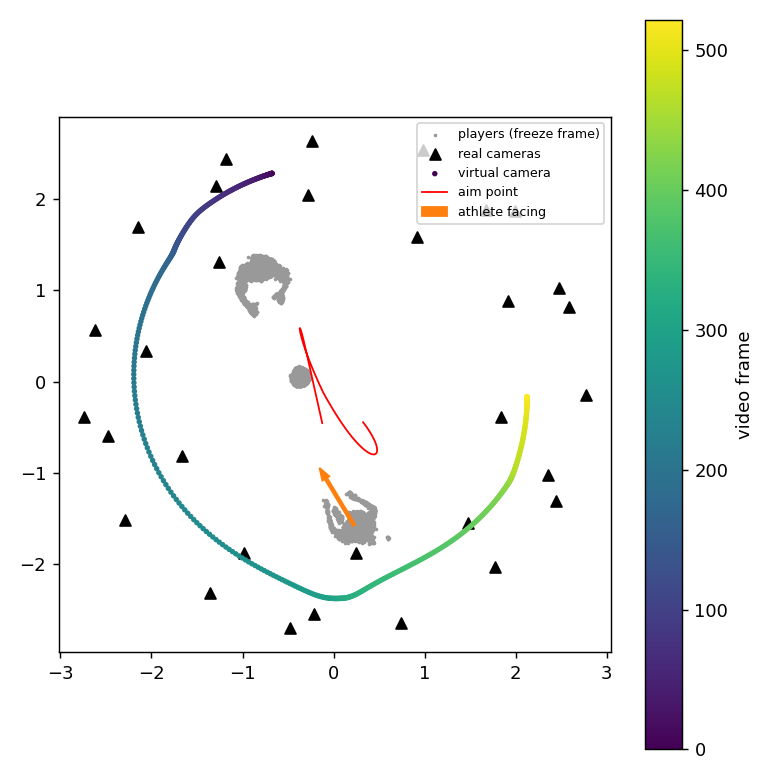
\includegraphics[width=0.92\columnwidth]{path_full.png}
\vspace{-0.8em}
\caption{\textbf{Planned camera path} for basketball, seen from above: players at the freeze frame (grey), real cameras (triangles), the virtual camera coloured by video frame, its aim point (red) and the key athlete's facing direction (arrow).}
\label{fig:path}
\vspace{-1em}
\end{figure}

\begin{figure}[t]
\centering
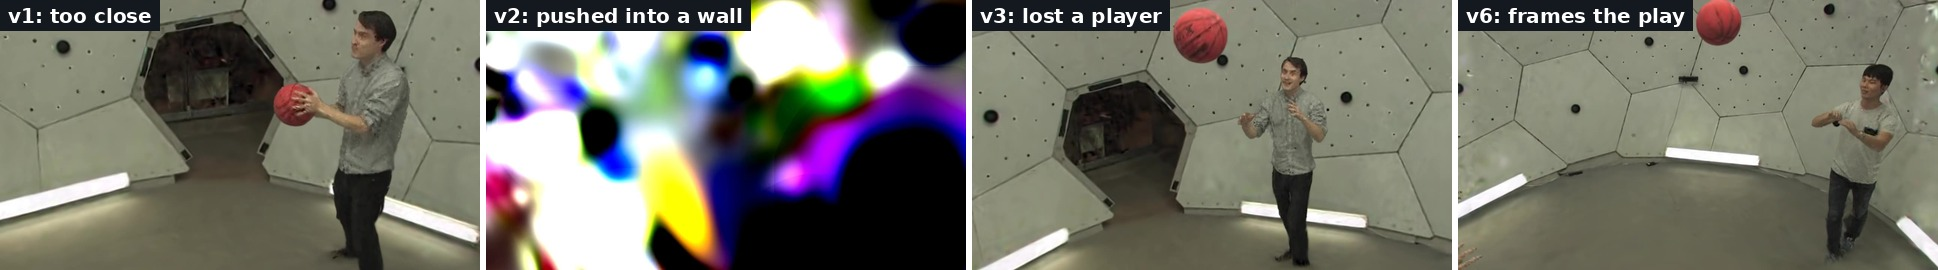
\includegraphics[width=\columnwidth]{director_versions.jpg}
\vspace{-1.6em}
\caption{\textbf{Why the rules exist} (mid-term, basketball). v1 flew too close; in v2 floaters pushed the camera into the wall; v3 dropped the second player; v6 follows the play.}
\label{fig:versions}
\vspace{-1em}
\end{figure}

\subsection{Q6: viewer study}
Numbers like jerk do not say what a viewer would put on air. We built a web page that shows two replays of the same play side by side, in sync, and asks which is better (A, B, or about the same), with optional reasons: smoother camera, better angle, better moment, sharper athlete, camera stays clear of players. Each viewer sees 8 pairs in a random order with random sides. Each pair sets the full director against one change: the mid-term v6, no smoothing, no clearance, or frame-repeat slow motion, in basketball and tennis. \pending{[Results pending: $N$ viewers, \% preferring the full director per pair, top reasons. To be filled from the study before submission.]}

\subsection{Which physical priors matter?}
\label{sec:priors}
D3G's three priors are meant to keep motion physical. We retrained basketball with each one switched off (\cref{tab:priors}). The result is a trade-off. Every prior \emph{lowers} held-out PSNR a little, but makes the 3D motion more correct. Without rigidity, mean track error rises from 9.2 to 13.4\cm, the median almost doubles, and torso error grows five-fold (2.9$\to$14.1\cm): neighbouring Gaussians drift apart while each still looks right in the images. Without rotation or isometry, arm error grows by 4--13\cm. A caution on the PSNR column: the priors only act from frame 1 on, so all four runs are identical at frame 0, yet they already differ by 1.2\dB there. This is run-to-run noise, and the PSNR gaps are of that size. The drop over the clip is similar for all four ($-0.6$ to $-1.0$\dB). So the priors' value shows up in 3D, which only a check against ground-truth motion can see.

\begin{table}[t]
\centering\small
\setlength{\tabcolsep}{3pt}
\begin{tabular}{lcc|cccc}
\toprule
& \multicolumn{2}{c|}{PSNR (dB)} & \multicolumn{4}{c}{track error (cm)}\\
Basketball & frame 0 & mean & mean & med. & torso & arms\\
\midrule
full D3G & 27.99 & 27.03 & \textbf{9.22} & \textbf{3.66} & \textbf{2.94} & 24.9\\
$-$ rigidity & 28.48 & 27.86 & 13.42 & 6.11 & 14.12 & \textbf{11.7}\\
$-$ rotation & 29.20 & 28.41 & 11.08 & 4.28 & 3.62 & 29.2\\
$-$ isometry & 28.59 & 27.68 & 11.91 & 3.77 & 3.00 & 37.8\\
\bottomrule
\end{tabular}
\vspace{-0.6em}
\caption{\textbf{Prior ablation.} Frame 0 is trained identically in all runs (priors start at frame 1), so its spread shows the run-to-run noise.}
\label{tab:priors}
\vspace{-1em}
\end{table}

%%%%%%%%%%%%%%%%%%%%%%%%%%%%%%%%%%%%%%%%%%%%%%%%%%%%%%%%%%%%%%%%%%%%%%
\section{Analysis: where does it fail?}
\label{sec:analysis}

\noindent\textbf{Does fast motion cause the error?} One would expect the model to struggle most when the athlete moves fast. It does not, at least not frame by frame. Correlating per-frame held-out PSNR with athlete speed gives $r$ between $-0.27$ and $+0.30$ across the six sports (\cref{fig:speed}). Instead, the worst frame of every clip is late (frames 106--148), and PSNR slides down slowly over the clip. Error builds up over time as each frame starts from the last, rather than spiking on fast frames. Speed does hurt where it matters most for a replay: the in-between frames (Q3), where the fastest clips, softball and tennis, lose the most with linear blending.

\noindent\textbf{What do failures look like?} \cref{fig:worst} shows each clip's worst frame next to the real view. The overall look holds up; the faults are local: speckled floaters near the box stack, a thinner, broken-up bat and racket, and softer hands. These match the track errors: arms and held objects are the hardest parts.

\begin{figure}[t]
\centering
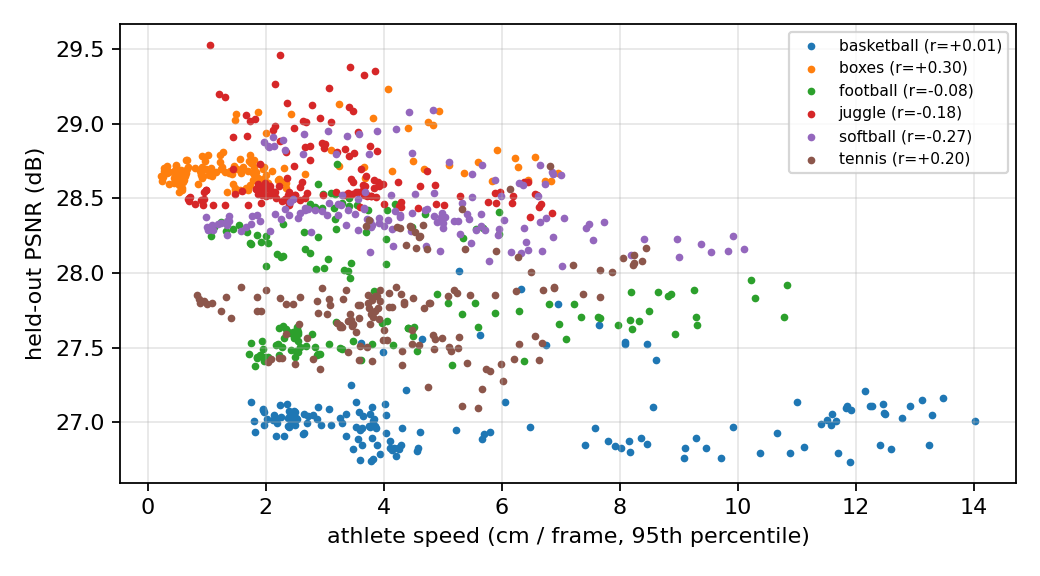
\includegraphics[width=\columnwidth]{psnr_vs_speed.png}
\vspace{-1.6em}
\caption{\textbf{Error vs.\ speed.} Per-frame held-out PSNR against athlete speed (95th-percentile Gaussian speed). The correlation is weak in every sport.}
\label{fig:speed}
\vspace{-1em}
\end{figure}

\begin{figure*}[t]
\centering
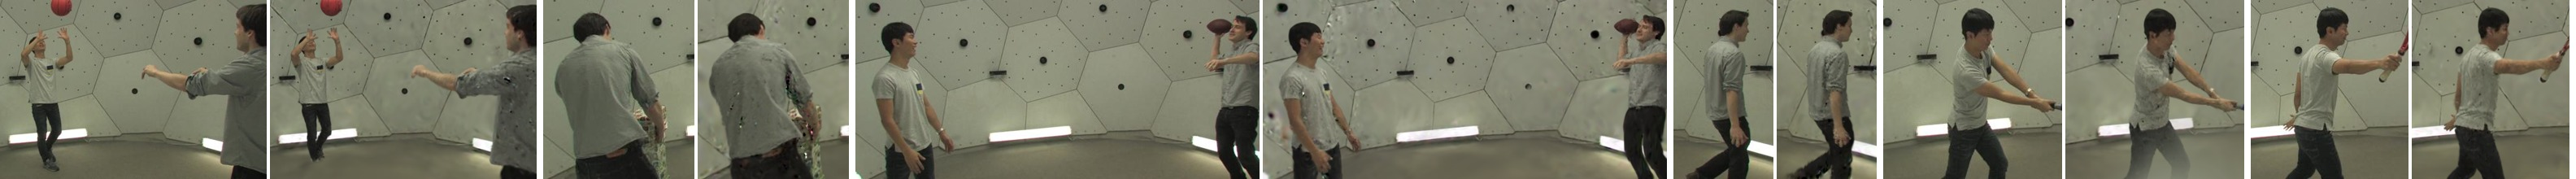
\includegraphics[width=\textwidth]{worst_frames.jpg}
\vspace{-1.6em}
\caption{\textbf{Worst held-out frame of each clip}, cropped to the athletes: real (left) and ours (right) in each pair. Basketball, boxes, football, juggle, softball, tennis.}
\label{fig:worst}
\vspace{-1em}
\end{figure*}

\noindent\textbf{Limitations.} (1) A lab dome is small, evenly lit and densely covered; a stadium is none of these, and its cameras would be calibrated by structure-from-motion, not a studio rig. (2) Each clip takes about 3 hours to train; a broadcast needs a replay in seconds, which points to feed-forward models (\cref{sec:related}). (3) Skeletons come from the studio here; in the wild they would come from a pose estimator, with more noise. (4) The key-moment rule only looks in the middle of the clip and confuses lifting with placing. (5) The viewer study is small and drawn from classmates.

%%%%%%%%%%%%%%%%%%%%%%%%%%%%%%%%%%%%%%%%%%%%%%%%%%%%%%%%%%%%%%%%%%%%%%
\section{Conclusion}
\label{sec:conclusion}

We built an open pipeline that turns synchronized multi-angle video into a cinematic 3D replay, and we tested each step on six sports with models we trained ourselves. The 4D models match unseen views (27--29\dB) and follow the athletes' joints to a few centimetres. Three additions fix the mid-term's weak spots. Skeleton cues find the key moment far better than the ball rule. A facing-aware path cuts back views by up to a third where the old rule failed. Cubic interpolation gives sharper slow motion, up to 1.5\dB better on the athlete. Two findings were less expected. D3G's priors trade a little image quality for much better 3D motion, which only ground-truth motion can reveal. And error builds up over time rather than with speed. Next steps are a faster, feed-forward model, skeletons from a pose estimator so the pipeline runs outside the studio, and an interactive viewer where the audience picks its own angle. Code: \url{https://github.com/sportsanalystf/free-viewpoint-athletes-d3g}.

{\small
\bibliographystyle{ieeenat_fullname}
\bibliography{main}
}
\end{document}
